\chapter{Messungen am Frequenzumformer}
\label{chap:Versuch}
In diesem Kapitel sollen der Messaufbau und die Auswertung der Messergebnisse des Frequenzumformers beschrieben werden. Mit Hilfe der Messungen wird dann in \cref{chap:VerfikationValidierung} das \textsc{Modelica}-Modell mit der elektrischen Anlage abgeglichen. Schließlich werden die Ergebnisse des ParameterSweeps in \cref{chap:Auswertung} mit den Ergebnissen der Messreihen verglichen. 

Aufgenommen wurden Zeitverläufe der Spannungen und Ströme an den Ein- und Ausgängen des Umformers, sowie am Ausgang des Spannungsreglers und des mitrotierenden Gleichrichters. Verwendet wurde dazu eine Standardmesseinrichtung mit Lastbank für Typ- und Serienprüfungen elektrischer Anlagen der Fa. Piller Power Systems. 

Im Folgenden wird zunächst dieser Messaufbau beschrieben. Anschließend folgt ein Überblick über die aufgenommenen Daten und deren Aufbereitung und Auswertung.

\section{Messaufbau}
\label{sec:Messaufbau}
Die Aufnahme der Messung wurde in Zusammenarbeit mit Mitarbeitern des Prüffelds der Firma Piller Power Systems durchgeführt. 
\begin{figure}
    \centering
    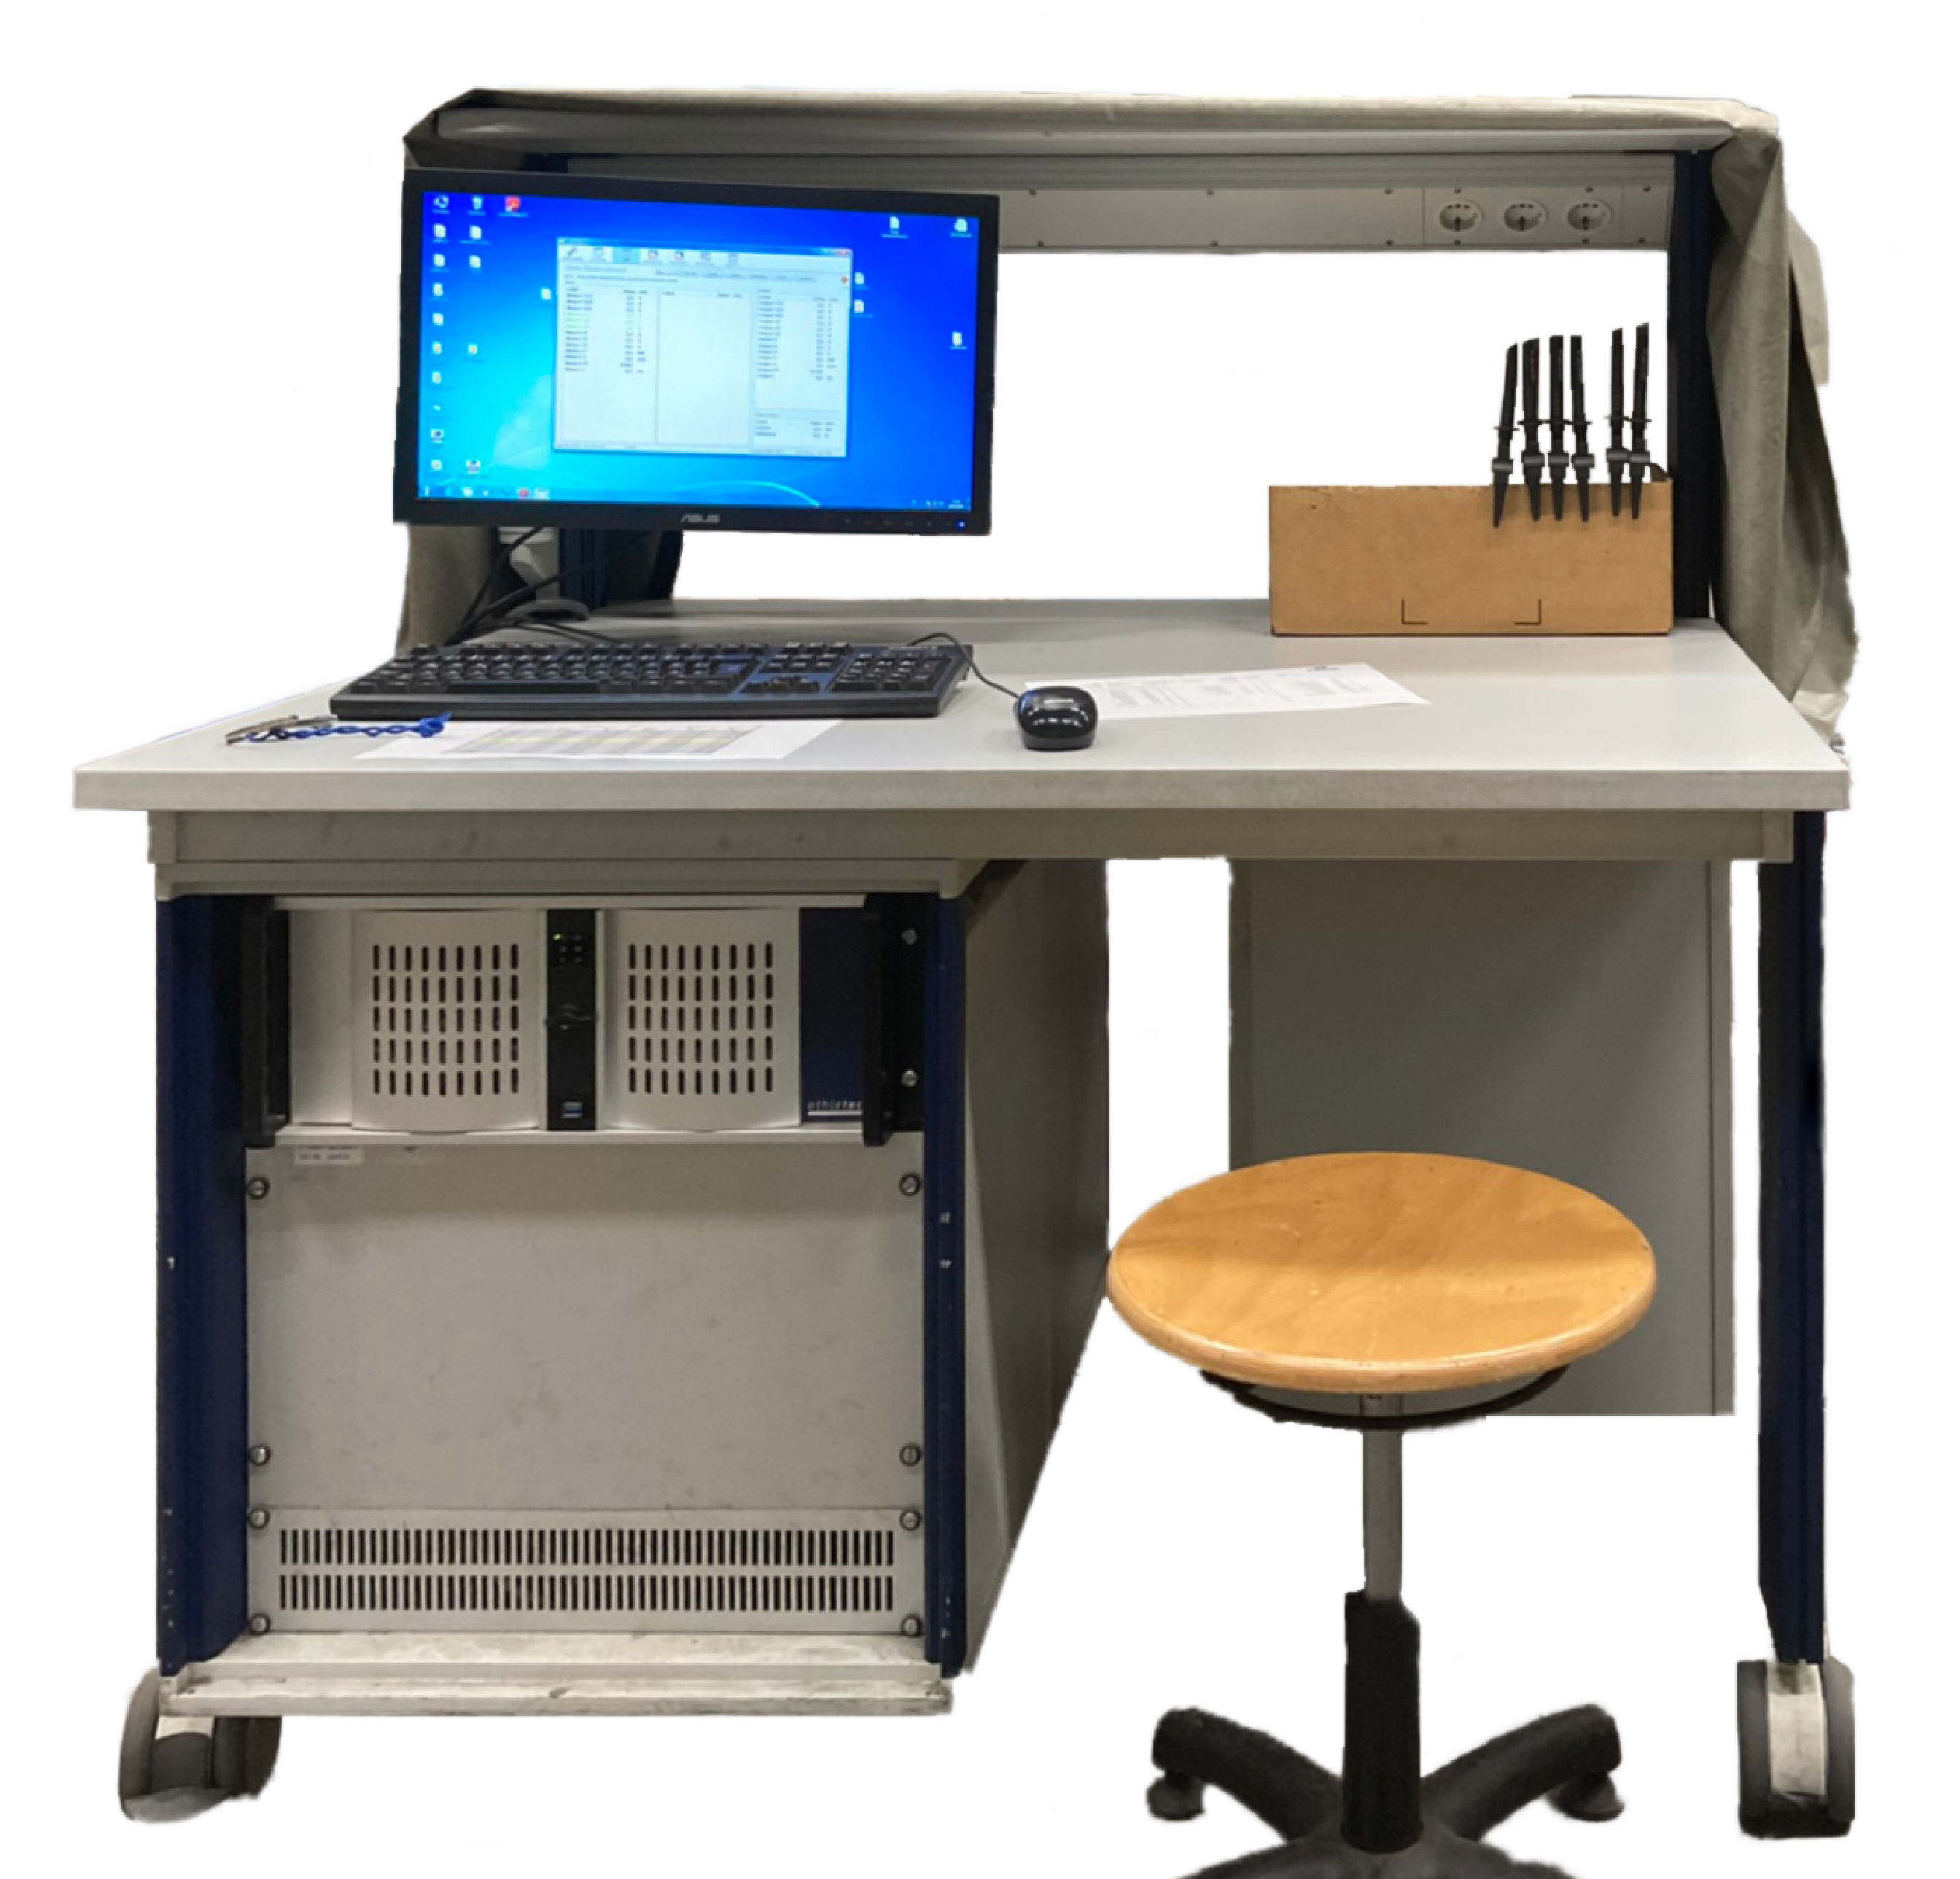
\includegraphics{Bilder/Messwagen vorne}
    \caption{Messwagen der Firma Piller Powers Systems (eigene Aufnahme)}
    \label{fig:Messwagen}
\end{figure}
Mit einem Messwagen (siehe \cref{fig:Messwagen}), bestehend aus Computer, Messkarte und Messsoftware und benötigten Wandlerschaltungen zum Anpassen der Messgrößen auf den Messbereich der Messkarte, wurden statische Werte und Zeitverläufe der Messgrößen ermittelt. Die dazu benötigte Belastung der Maschine wurde über eine Lastbank aus schaltbaren Widerständen und Induktivitäten eingestellt. Die Einstellung erfolgte über Schalten der Last und direktes Vergleichen der resultierenden Scheinleistung und des resultierenden Leistungsfaktor am Messsytem. Eingestellt wurden jeweils Lasten in Prozent mit Bezug auf die Nennscheinleistung der Anlage. 

\begin{figure}
    \centering
    \begin{subfigure}[t]{.3\textwidth}
         \centering
         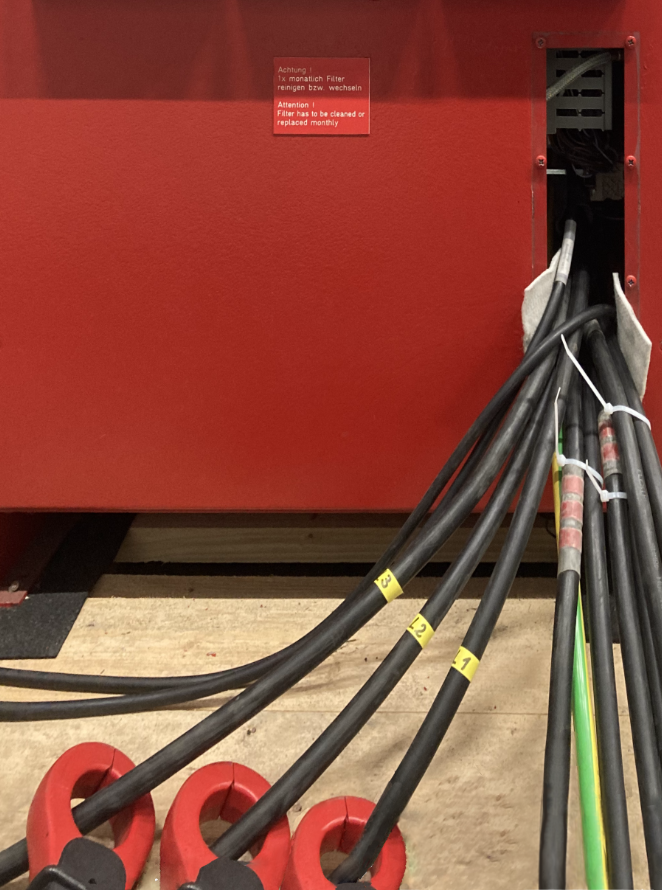
\includegraphics[height=5cm]{Bilder/Stromzangen.png}
         \caption{Stromzangen am Lastausgang}
         \label{fig:Umformer_Stromzangen}
     \end{subfigure}\hfill%
    \begin{subfigure}[t]{.4\textwidth}
          \centering
          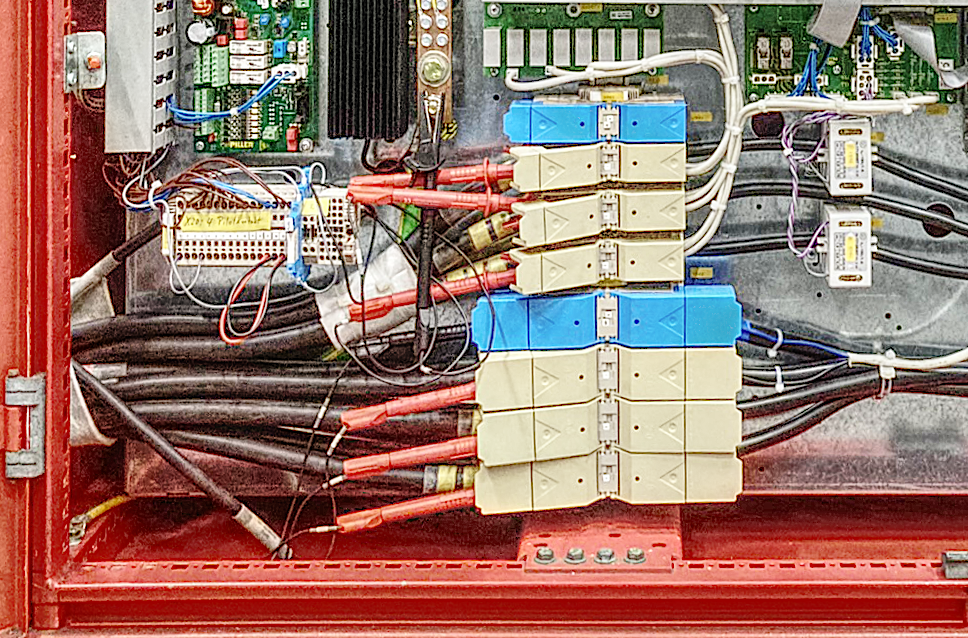
\includegraphics[height=5cm]{Bilder/Klemmen.png}
          \caption{Klemmen zur Spannungsmessung}
          \label{fig:Umformer_vorne}
     \end{subfigure}\hfill%
     \begin{subfigure}[t]{.2\textwidth}
          \centering
          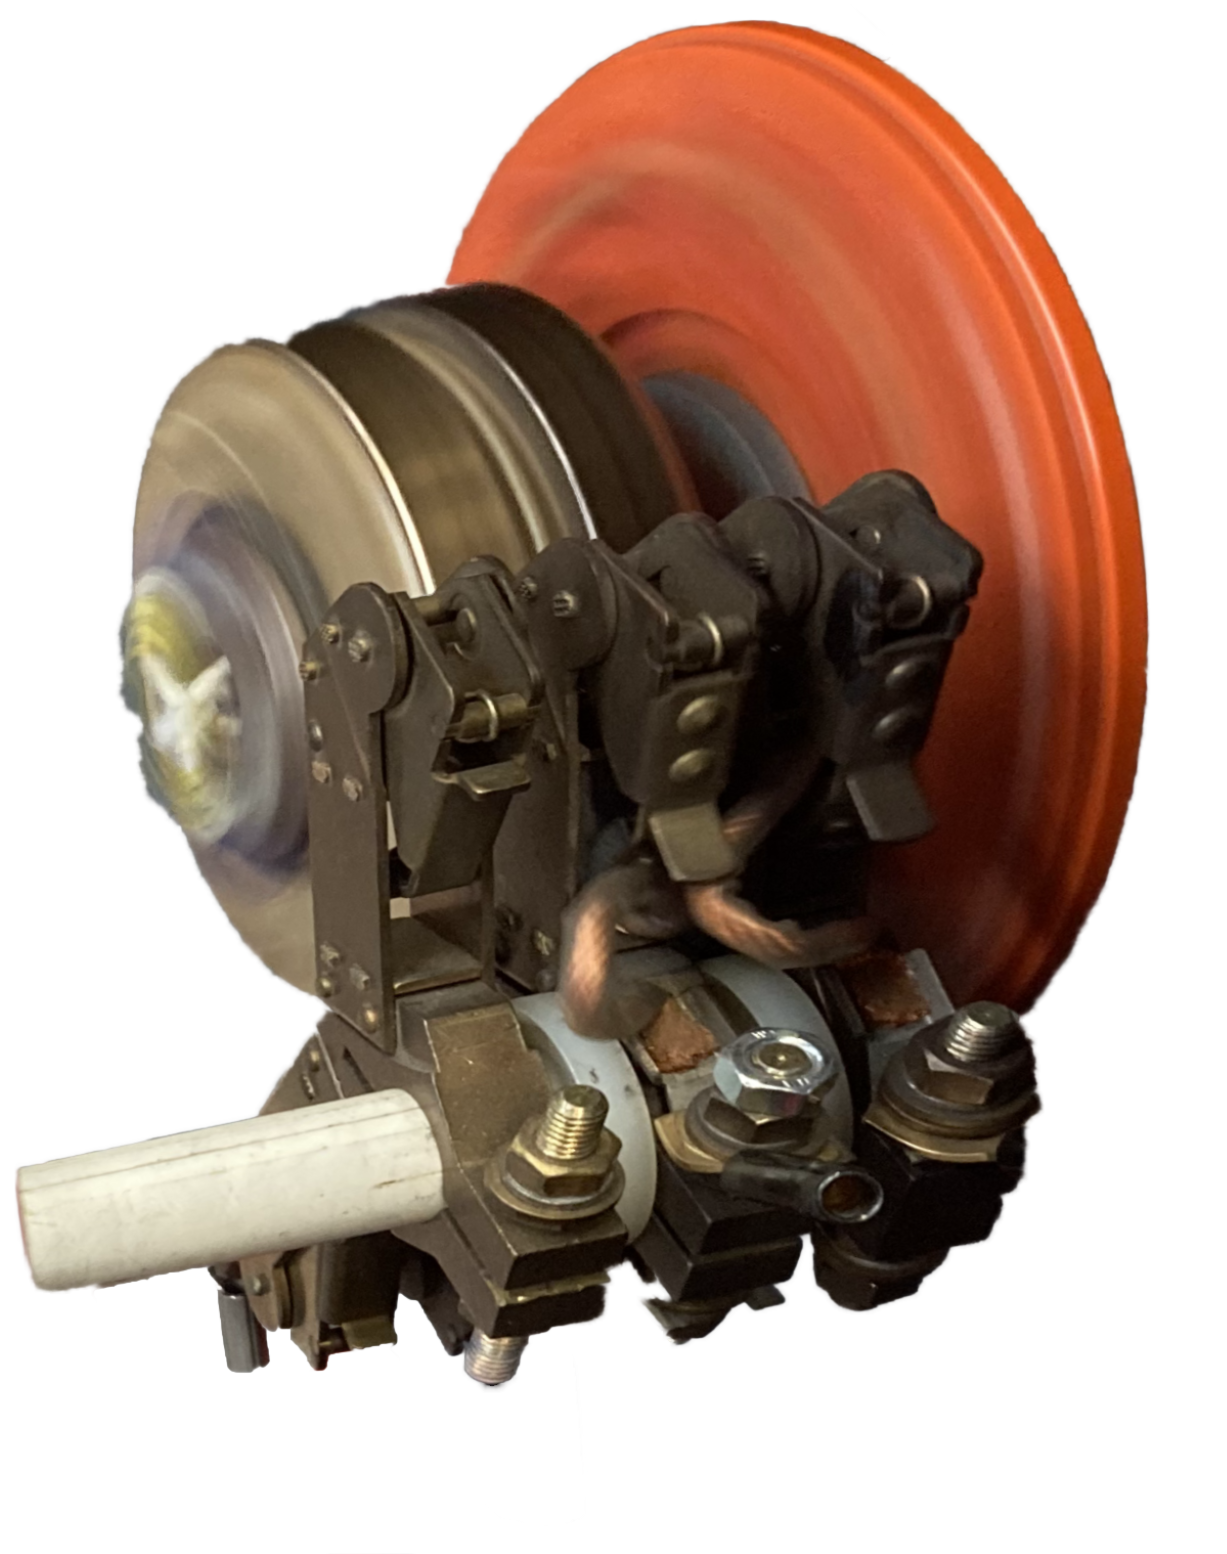
\includegraphics[]{Bilder/Polrad_freigestellt.png}
          \caption{Schleifringe und Diodenrad}
          \label{fig:Umformer_Polrad}
     \end{subfigure}\hfill%
    \caption{Umformer mit Messanschlüssen (eigene Aufnahmen)}
    \label{fig:Messaufbau}
\end{figure}

Die aufgenommenen Messgrößen sind die drei Strom- und Spannungsphasen des Netzeingangs und des Ausgangs der Anlage, der Strom und Spannungsausgang am Spannungserzeuger des Reglers und die gleichgerichtete Spannung am Ausgang des auf dem Polrad mitrotierenden Gleichrichters (\emph{Haupterregerspannung}). Gefahren wurden drei Arten von Messläufen: \begin{enumerate}
    \item Statische Messung: Ein kurzer Zeitabschnitt der Messgrößen wurde mit den Lasten $[\unit[0]{\%}, \unit[25]{\%}, \unit[50]{\%}, \unit[75]{\%}, \unit[100]{\%}, \unit[125]{\%}, \unit[150]{\%}]$ der Nennscheinleistung jeweils bei einem Leistungsfaktor von $\mathrm{Pf} = 1$ und $\mathrm{Pf} = 0{,}8$ aufgenommen. Die Messung bei $\unit[0]{\%}$~Last fand jedoch nur bei $\mathrm{Pf}=1$ statt.
    \item Dynamische Messung: Die Messgrößen wurden für ca $\unit[10]{s}$ aufgezeichnet. Während der Messung wurde ein Lastsprung ausgeführt, für jeden Sprung jeweils ein Aufschalten und ein Abwurf der Last und ebenfalls jeweils mit einem Leistungsfaktor von $\mathrm{Pf}=1$ und $\mathrm{Pf}=0{,}8$. Vermessen wurden die Lastsprünge $[\unit[0]{\%}, \unit[50]{\%}]$, $[\unit[0]{\%}, \unit[100]{\%}]$ und $[\unit[50]{\%}, \unit[100]{\%}]$.
    \item Dynamische Messung mit Veränderung der Reglerparameter: Wie bei der Dynamischen Messung ohne Veränderung der Reglerparameter wurden die Messgrößen für ca $\unit[10]{s}$ während eines Lastsprungs aufgenommen, jedoch mit veränderten Reglerparametern. Die eingestellten Parameter können den \cref{tab:Parameter-D-Messung,tab:Parameter-I-Messung,tab:Parameter-P-Messung,tab:Parameter-PI-Messung} im Anhang entnommen werden. Die Lastsprünge (Aufschalten und Abwurf) wurden bei $[\unit[50]{\%}, \unit[100]{\%}]$ Last und einem Leistungsfaktor von $\mathrm{Pf}=0,8$ ausgeführt.
\end{enumerate}

Die Ströme wurden mit Stromzangen (siehe \cref{fig:Umformer_Stromzangen}) an den Zu- und Ableitungen gemessen, die Ein- und Ausgangsspannungen und die Reglerspannung wurden mit entsprechenden Klemmen im Frequenzumformer aufgenommen (siehe \cref{fig:Umformer_vorne}). Die gleichgerichtete Haupterregerspannung wurde über dafür montierte Schleifringe von der Welle abgeführt (\cref{fig:Umformer_Polrad}). Mit der Messsoftware wurden die Messdaten aufgezeichnet und wegen der höheren Schreibgeschwindigkeit in einem Binärformat abgespeichert. Für die weitere Verarbeitung wurden die Messwerte anschließend in das Textformat \texttt{.csv} umgewandelt. Die Aufzeichnung der transienten Größen erfolgte mit einer Abtastrate von $f_{\mathrm{s}}=\unit[60]{kHz}$.

\section{Aufbereitung der Messergebnisse}
\label{sec:Auswertung_Messeregbnisse}
Die Aufbereitung der Messergebnisse erfolgte in einem Jupyter-Notebook mit Python und einem ergänzenden Python-Modul \texttt{preprocessData.py}. Der entwickelte Quellcode ist im Anhang unter \cref{lst:PreprocessData} zu finden.

%Die Auswertung der Messergebnisse unterteilte sich in zwei Phasen: Zuerst mussten die Daten aufbereitet werden, Verläufe geglättet und Leistung, Frequenzen und Effektivwerte der elektrischen Größen bestimmt werden. Im nächsten Schritt konnten dann die Kenndaten der elektrischen Anlage und der einzelnen Maschinen gewonnen und zum Abgleich mit dem Modelica-Modell vorbereitet werden. 

Mit dem Modul wurden aus den eingelesenen Daten die folgenden Größen in dieser Reihenfolge bestimmt:
\begin{itemize}
    \item Leiter-Leiter-Spannungen aus den gemessenen Leiter-Neutralleiterspannungen: 
        \begin{equation}
        x_{\mathrm{LL}} = x_{\mathrm{2\,LN}} - x_{\mathrm{1\,LN}}
        \end{equation}
    \item Frequenzen der Größen: Da die betrachteten Strom- und Spannungsverläufe die Sinusform gut annähern, konnten die Periodenlängen bzw. Frequenzen durch Erkennen der Nulldurchgänge (\emph{Zero-Crossing}) ermittelt werden.
    \item Effektivwerte der Größen, ermittelt jeweils über eine Periode mit \begin{equation}
        X_{\mathrm{eff}}=\sqrt{\mathrm{mean}(x^2)},
    \end{equation}
    wobei $\mathrm{mean}(x)$ als der arithmetische Mittelwert gemäß \begin{equation}
        \mathrm{mean}(x) \coloneqq \frac{1}{n} \sum_{i=1}^n x_i
    \end{equation}
    definiert ist.
    \item Scheinleistung am Ein- und Ausgang, jeweils über eine Periode ermittelt nach \begin{equation}
		S_i = u_i \cdot i_i
    \end{equation}
    \item {Gleitender Mittelwert des Stroms und der Spannung am Ausgang des Reglers. Gemittelt wurde über 10 Perioden mit einer Frequenz von $f=\unit[2500]{Hz}$, die aus den Rohdaten für die Pulse abgelesen wurde.
    }
\end{itemize}
Anschließend wurden die Datenreihen jeweils über 10 Perioden mit einem gleitenden Mittelwert geglättet (bzw. über $\Delta T_{\mathrm{mittel}}=\frac{10}{\unit[2500]{Hz}}=\unit[4]{ms}$ im Falle der Reglerausgangsgrößen). Zur weiteren Auswertung wurden die Messgrößen als Spalten in einem Pandas-\texttt{Dataframe} angeordnet und, um Wartezeiten durch erneutes Einlesen der Daten zu vermeiden, als binäres Speicherabbild gesichert. \Cref{sec:ReglerparameterDynamischeMessung,sec:MessergebnisseOhneRegleranderung} zeigen die Ergebnisse der statischen und dynamischen Messung mit und ohne Reglerveränderung.
